\begin{pastexam}[label={px:ust-114-ee-ds-22}]{臺聯大電機類 114 學年度 第 22 題}
（複選；5 分，答錯倒扣 1 分，倒扣至本大題 0 分為止）

Height: Assume that the height of a tree node is the number of edges on the longest path from the
node to a leaf. A leaf node will have a height of 0. Balance: The balance of a node is defined:
left\_child\_node's height - right\_child\_node's height. The balance of a leaf node is 0 (since The
height of a ``None'' child node is defined as -1).

\begin{center}
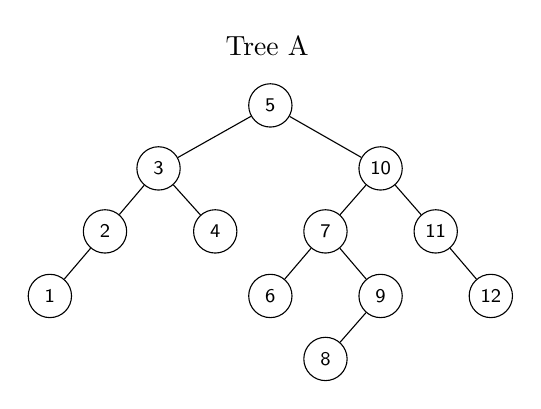
\begin{tikzpicture}[n/.style={circle,draw,inner sep=0pt,minimum size=5.5mm,font=\scriptsize\sffamily}]
\node at (2.76,0.75) {Tree A};
\node[n] (n5) at (2.80,0.00) {5};
\node[n] (n3) at (1.38,-0.80) {3};
\node[n] (n10) at (4.20,-0.80) {10};
\node[n] (n2) at (0.70,-1.60) {2};
\node[n] (n4) at (2.10,-1.60) {4};
\node[n] (n7) at (3.50,-1.60) {7};
\node[n] (n11) at (4.90,-1.60) {11};
\node[n] (n1) at (0.00,-2.42) {1};
\node[n] (n6) at (2.80,-2.42) {6};
\node[n] (n9) at (4.20,-2.42) {9};
\node[n] (n12) at (5.60,-2.42) {12};
\node[n] (n8) at (3.50,-3.22) {8};
\draw (n5)--(n3);
\draw (n5)--(n10);
\draw (n3)--(n2);
\draw (n3)--(n4);
\draw (n2)--(n1);
\draw (n10)--(n7);
\draw (n10)--(n11);
\draw (n7)--(n6);
\draw (n7)--(n9);
\draw (n9)--(n8);
\draw (n11)--(n12);
\end{tikzpicture}\hspace{1.2em}%
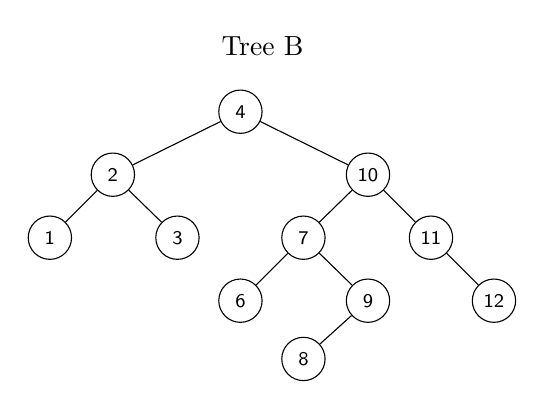
\begin{tikzpicture}[n/.style={circle,draw,inner sep=0pt,minimum size=5.5mm,font=\scriptsize\sffamily}]
\node at (2.70,0.75) {Tree B};
\node[n] (n4) at (2.42,-0.08) {4};
\node[n] (n2) at (0.80,-0.88) {2};
\node[n] (n10) at (4.04,-0.88) {10};
\node[n] (n1) at (0.00,-1.68) {1};
\node[n] (n3) at (1.62,-1.68) {3};
\node[n] (n7) at (3.22,-1.68) {7};
\node[n] (n11) at (4.84,-1.68) {11};
\node[n] (n6) at (2.42,-2.48) {6};
\node[n] (n9) at (4.04,-2.48) {9};
\node[n] (n12) at (5.64,-2.48) {12};
\node[n] (n8) at (3.22,-3.22) {8};
\draw (n4)--(n2);
\draw (n4)--(n10);
\draw (n2)--(n1);
\draw (n2)--(n3);
\draw (n10)--(n7);
\draw (n10)--(n11);
\draw (n7)--(n6);
\draw (n7)--(n9);
\draw (n9)--(n8);
\draw (n11)--(n12);
\end{tikzpicture}
\end{center}

Which of the following statements are true based on the definitions given above. (5\%) multiple
anwsers
\begin{enumerate}[label=(\Alph*)]
\item The balance of every node in Tree A is 1, 0, or -1.
\item The balance of every node in Tree B is 1, 0, or -1.
\item Tree A is a binary search tree
\item Tree B is a binary search tree
\item Both Tree A and Tree B are AVL trees.
\end{enumerate}
\end{pastexam}

\begin{pastsoln}
答案是 (A)(C)(D)。

照題目的定義（高度用邊數，空子樹高度 $-1$）由下往上算。 記 $h$ 為高度、$b$ 為 balance。

\textbf{Tree A}：葉節點 1、4、6、8、12 的 $h = 0$、$b = 0$。
\begin{center}
\small
\begin{tabular}{cccc}
\toprule
節點 & 左子樹高度 & 右子樹高度 & $h$，$b$ \\
\midrule
9 & 0（8） & $-1$ & $1$，$+1$ \\
2 & 0（1） & $-1$ & $1$，$+1$ \\
11 & $-1$ & 0（12） & $1$，$-1$ \\
7 & 0（6） & 1（9） & $2$，$-1$ \\
3 & 1（2） & 0（4） & $2$，$+1$ \\
10 & 2（7） & 1（11） & $3$，$+1$ \\
5 & 2（3） & 3（10） & $4$，$-1$ \\
\bottomrule
\end{tabular}
\end{center}
每個節點的 $b$ 都在 $\{1, 0, -1\}$ 裡。

\textbf{Tree B}：右半邊（10 這棵子樹）和 Tree A 相同，10 的 $h = 3$、$b = +1$；2 的子節點是 1、3，
$h = 1$、$b = 0$。 根 4：左子樹高度 $1$、右子樹高度 $3$，$b = 1 - 3 = -2$。

\textbf{是不是二元搜尋樹}：看中序是否遞增（資結書定理~9.1）。 Tree A 的中序是
$1, 2, 3, 4, 5, 6, 7, 8, 9, 10, 11, 12$；Tree B 的中序是 $1, 2, 3, 4, 6, 7, 8, 9, 10, 11, 12$
（沒有 5，但仍遞增）。 兩棵都是二元搜尋樹。 例如 8 在 9 的左邊、在 7 的右子樹裡，$7 < 8 < 9$，沒問題。
\begin{itemize}
\item (A)：見表，對。
\item (B)：根 4 的 balance 是 $-2$。 錯。
\item (C)(D)：中序遞增，對。
\item (E)：AVL 樹要是二元搜尋樹而且每個節點 balance 在 $\{-1, 0, 1\}$（資結書第~10.2~節）。 Tree A 是，
Tree B 的根不是，所以「兩棵都是」錯。
\end{itemize}
\end{pastsoln}
